\documentclass{mwhittaker}
\title{Deep RL Assignment 3}
\date{October 4, 2017}

\usepackage{graphicx}

\newcommand{\tabref}[1]{Table~\ref{tab:#1}}
\newcommand{\figref}[1]{Figure~\ref{fig:#1}}

\begin{document}
\maketitle

\section*{Question 1: basic Q-learning performance}
\begin{figure}[h]
  \centering
  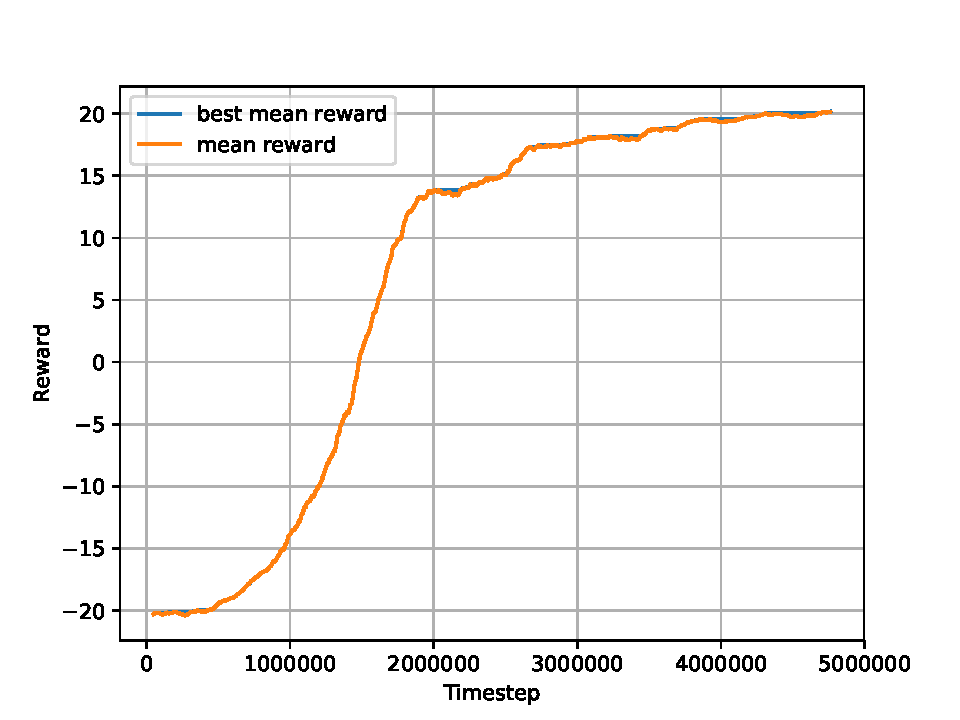
\includegraphics[width=\textwidth]{q1.pdf}
  \caption{%
    The mean 100-episode reward and best mean reward of a DQN trained policy
    running Pong. All default hyperparameters were used. A score of 20 was
    reached around timestep 4.5 million.
  }\label{fig:q1}
\end{figure}

\clearpage

\section*{Question 2: experimenting with hyperparameters}
\begin{figure}[h]
  \centering
  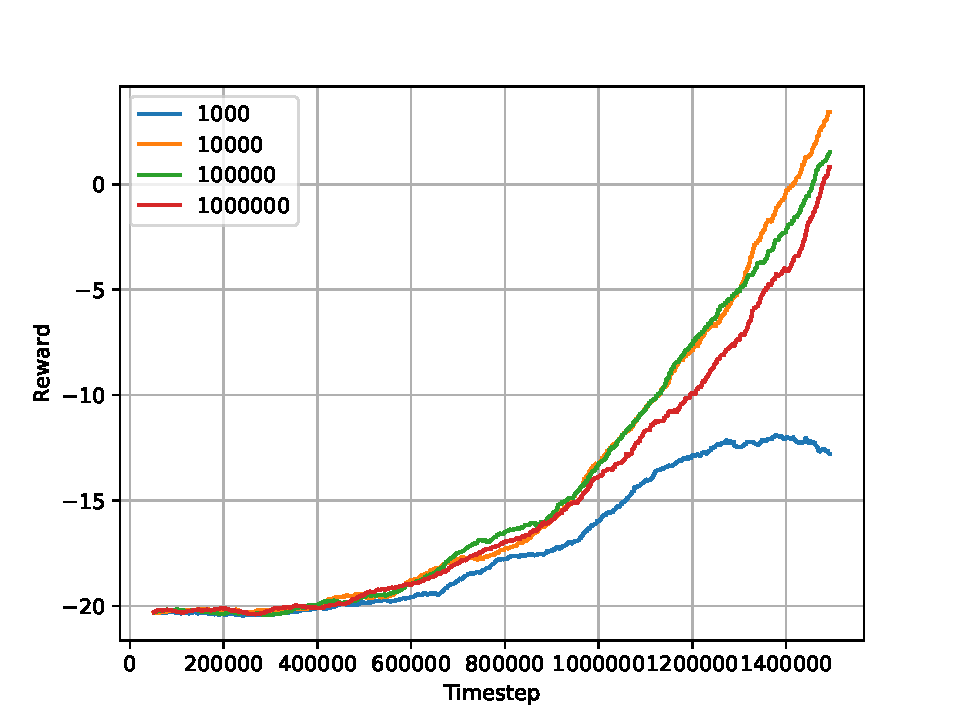
\includegraphics[width=\textwidth]{q2.pdf}
  \caption{%
    The blue, orange, green, and red lines show the mean reward of a DQN policy
    trained with a replay buffer of size 1,000, 10,000, 100,000, and 1,000,000
    respectively. I chose to vary the replay buffer size for two reasons.
    First, the default buffer size of 1,000,000 made the replay buffer too big
    to fit in RAM on my laptop. I wanted to know if smaller buffer sizes could
    produce comparable results. Second, I wanted to see if a smaller buffer
    could potentially increase the performance of the model by discarding old
    and somewhat irrelevant states. The figure shows that if the buffer is too
    small, the model does not train well. On the other hand, we can shrink the
    buffer by two orders of magnitude and achieve better performance after 1.5
    million timesteps.
  }\label{fig:q2}
\end{figure}

\end{document}
